\subsection{Validation}

Our validation framework assesses both the precision (consistency across multiple runs) and accuracy (comparison with expert-created matrices) of the LLM-driven model construction process. This dual approach provides comprehensive insights into the framework's reliability and ecological validity. We used four distinct Australian marine regions for these assessments: three regions (Northern Australia, South East shelf, and South East Offshore) to evaluate precision, and one region (Great Australian Bight) to evaluate accuracy.

We executed model generation across three distinct phases. In phase one, we established baseline configurations for each study region by processing species occurrence data and downloading relevant species data. In phase two, where the LLM is first called, we executed five independent iterations per region, maintaining fixed input parameters while allowing the LLM's stochastic decision processes to generate variation in outputs. In phase three, we conducted detailed statistical analyses of both precision across iterations and accuracy compared to expert-created matrices.

For the precision assessment, we calculated the Jaccard similarity coefficients between all possible pairs of iterations and analysed the coefficient of variation in diet proportions. For the accuracy assessment, we averaged the diet proportions of the five LLM-generated matrices and compared the resulting matrix with an expert-created matrix for the Great Australian Bight ecosystem (C. Bulman pers. comm.) that was used to inform \citep{Fulton2018}.

\subsubsection{Study Regions}

\begin{figure}[htbp]
    \centering
    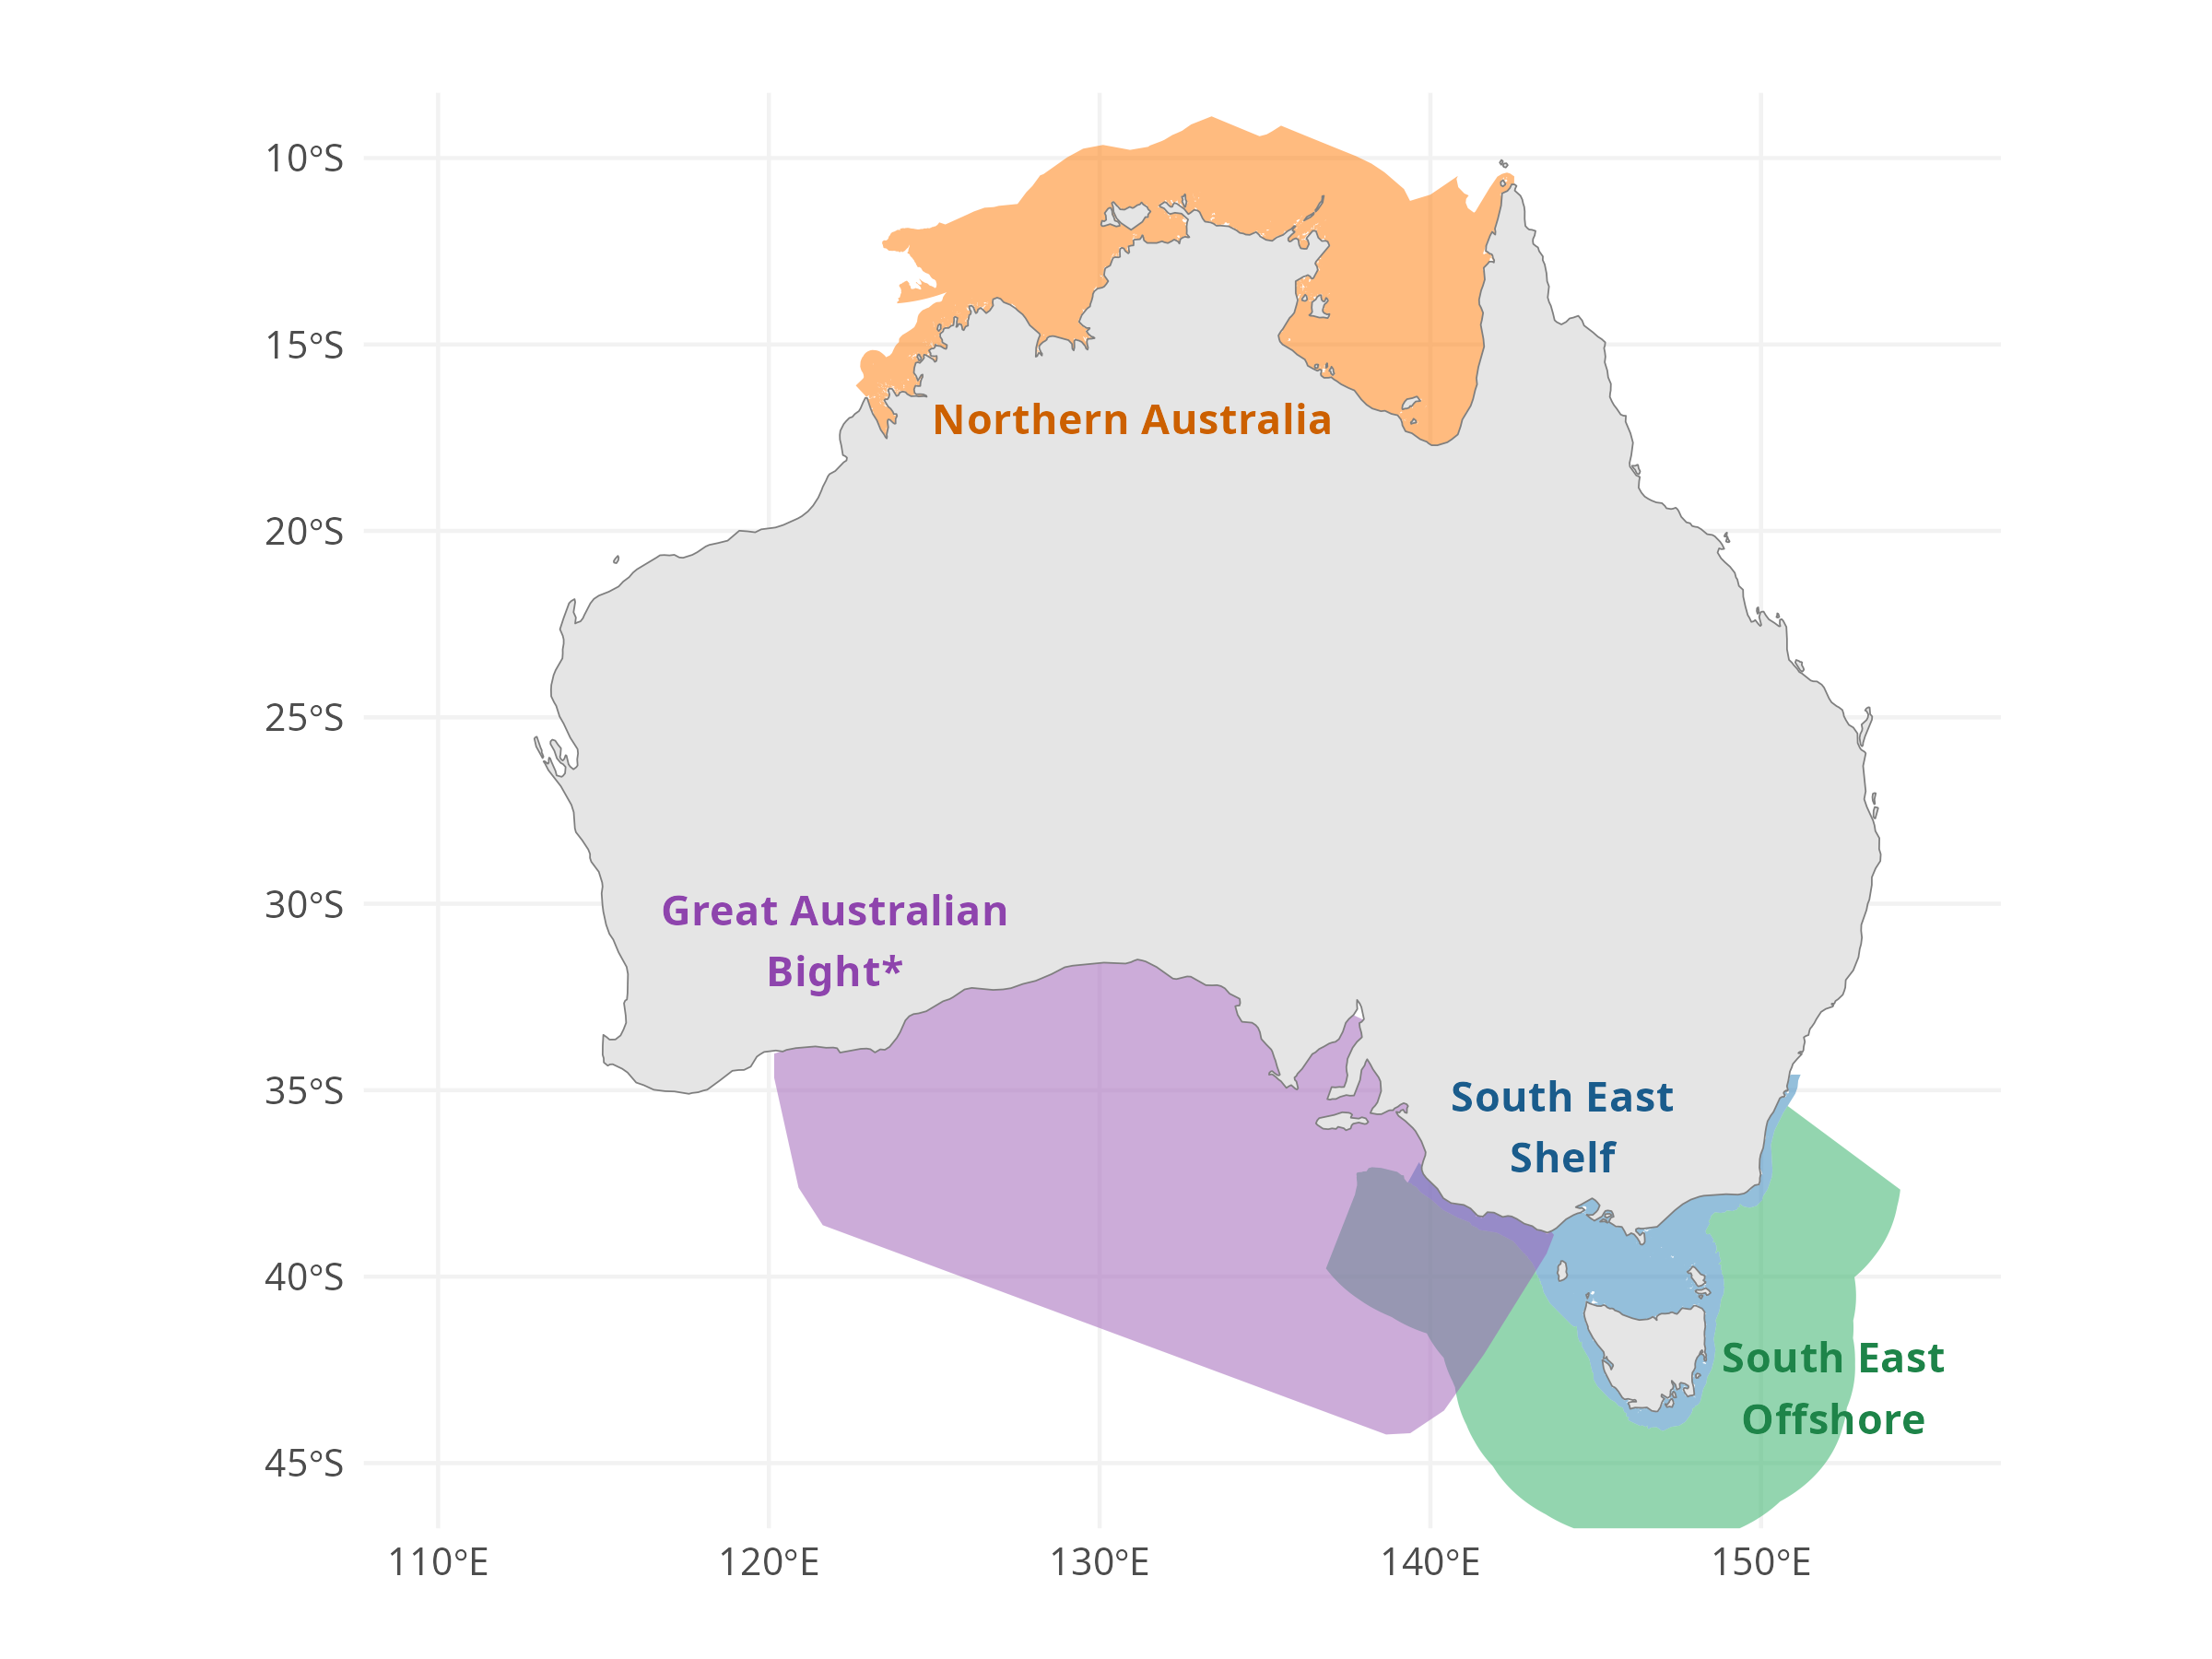
\includegraphics[width=0.8\textwidth]{figures/validation_regions.png}
    \caption{Map of the four study regions used to validate our approach: three of the regions were used to test the precision (consistency) of the approach: Northern Australia (orange), South East shelf (blue), South East Offshore (green). We used the fourth region, the Great Australian Bight (purple) to test the accuracy of our approach by comparing it to the initial diet matrix used in \citep{Fulton2018}}
    \label{fig:validation_regions}
    \end{figure}

We selected four Australian marine regions that present distinct ecological characteristics and modelling challenges for our framework (Figure \ref{fig:validation_regions}). For precision assessment, we used three regions: the Northern Australia region, which represents a tropical ecosystem characterised by a broad shelf and complex mix of reef systems, seagrass meadows, mangrove forests and bare sediment communities with seasonal monsoon influences; the South East shelf region, a temperate coastal system with a network of rocky reefs and kelp forests, rapidly changing environmental conditions due to climate change, comprehensive diet information in established databases, well-documented EwE models spanning multiple years, and active research programs; and the South East Offshore region, a deep-water ecosystem that challenges the framework with data-limited conditions and unique ecological patterns relating to oceanic through flow, shifting current patterns, low productivity patches interspersed with production concentrating canyons and seamounts.

For accuracy assessment, we used the fourth region: the Great Australian Bight (GAB), which represents a region of high conservation significance spanning diverse habitats. The GAB has been extensively studied, with research characterising the shelf and slope ecosystems from phytoplankton through to marine mammals and birds \citep{goldsworthy2013trophodynamics, Fulton2018}. We used this region to compare the resulting diet matrix from our process to the expert-created matrix used in \citep{Fulton2018}, allowing us to evaluate the accuracy of our approach.

The contrasting characteristics of these four regions provide a robust test of the framework's adaptability across different ecological contexts.

\subsubsection{Grouping Precision Analysis}

To assess the precision of AI-generated species groupings, we developed quantitative measures of grouping precision. For each of the three regions used for precision assessment (Northern Australia, South East shelf, and South East Offshore), we conducted five independent iterations, resulting in five grouping outcomes per region. We analyzed precision within each region separately.

For each region, we tracked each species' group assignments across the five iterations and calculated a precision score:

\[
\text{Precision Score} = \frac{\text{Number of occurrences in most common group}}{\text{Total number of iterations (5)}}
\]

This metric quantifies the framework's decision-making reliability for individual species within a specific ecological context. We classified species with precision scores below 1.0 as unstable, indicating variable group assignments across iterations. A species with a precision score of 1.0 was assigned to the same functional group in every iteration, demonstrating high precision in the framework's decision-making.

While the precision score measures stability at the individual species level, we also needed to evaluate stability at the group level. To do this, we assessed group stability using the Jaccard similarity coefficient between all possible pairs of iterations within each region:

\[
J(i,j) = \frac{|M_{i} \cap M_{j}|}{|M_{i} \cup M_{j}|}
\]

where $M_{i}$ and $M_{j}$ represent the sets of species members in iterations $i$ and $j$. Unlike the precision score, which focuses on whether individual species are consistently assigned to the same group, the Jaccard similarity measures whether a group consistently contains the same set of species across iterations. For example, a group might maintain a stable core of species while experiencing minor variations in peripheral members, which would be captured by the Jaccard similarity but not by individual species precision scores.

For each region, we calculated the overall stability score by averaging Jaccard similarities across all possible pairs of iterations. This approach reveals how consistently the framework identifies and maintains ecologically meaningful groupings across different runs. One-way ANOVA tests on these stability measures across regions, supplemented with Cohen's f effect size calculations, demonstrate the framework's precision across different marine ecosystems while maintaining consistent decision-making patterns.

\subsubsection{Grouping Accuracy Assessment}
\label{sec:taxonomic_accuracy}
To assess the ecological validity of AI-assigned functional groups, we conducted a manual validation of taxonomic grouping decisions. We did not use the original expert groupings from \citep{Fulton2018} for two reasons: first, the AI system handled many more taxonomic groupings and species than the human-created groupings, and second, comprehensive data for each functional group was no longer avaialable to do a direct comparison. Therefore, we undertook a direct evaluation where the lead author, SS, reviewed each taxonomic entity (ranging from species to higher taxonomic levels) for a single iteration of the GAB (n=675 AI-decisions) and evaluated whether the AI system had correctly assigned it to an appropriate functional group based on known ecological characteristics.

For each taxonomic group assigned by the AI system to a functional group, we researched the known ecological characteristics of that taxon, including feeding behavior, habitat preferences, and trophic position. We compared these ecological characteristics to the description of the functional group provided in the grouping template. Based on this comparison, we classified each assignment as either "Correct" (the taxon fits well within the functional group), "Partial" (the taxon partially fits the functional group but has some characteristics that don't align), "Incorrect" (the taxon was inappropriately assigned), or "Not Sure" (insufficient information was available to make a determination).


\subsubsection{Diet Matrix Precision Assessment}
To evaluate the precision of AI-generated trophic interactions and assess the framework's ability to capture distinct ecological patterns, we developed a multi-metric analysis approach. For each region separately (with five iterations per region), we calculated the following metrics for each predator-prey interaction:

\begin{enumerate}
    \item Presence ratio across iterations:
    \[
    P_{ij} = \frac{\text{Number of iterations with interaction}}{n}
    \]
    where $n$ is the total number of iterations (5 per region), and an interaction is present when the diet proportion $x_{ijk} > 0$ for predator $i$ consuming prey $j$ in iteration $k$.

    \item Mean diet proportion:
    \[
    \mu_{ij} = \frac{1}{n}\sum_{k=1}^{n} x_{ijk}
    \]
    where $x_{ijk}$ represents diet proportion for predator $i$ consuming prey $j$ in iteration $k$.

    \item Stability score:
    
    We first calculate a normalized deviation score for each predator-prey interaction:
    \[
    D_{ij} = \frac{1}{n}\sum_{k=1}^{n} \frac{|x_{ijk} - \mu_{ij}|}{\max_{k}(|x_{ijk}|)}
    \]
    
    where $\mu_{ij}$ is the mean diet proportion across iterations, and $\max_{k}(|x_{ijk}|)$ is the maximum absolute value across iterations. Because diet proportions ($x_{ijk}$) are bounded between 0 and 1, this deviation score ranges from 0 to 0.5.
    
    Then, to create a more intuitive stability score where higher values represent greater stability, we invert this measure:
    \[
    S_{ij} = 1 - D_{ij}
    \]
    
    This transformation yields a stability score bounded between 0.5 (maximum instability) and 1 (perfect stability), with higher values indicating more consistent diet proportions across iterations.
\end{enumerate}

We chose this stability metric over traditional variance measures for several reasons. First, by normalizing deviations by the maximum value, the metric achieves scale independence, allowing meaningful comparisons between interactions of different magnitudes. For example, the sequences [0.2, 0.2, 0.2, 0.2, 0.1] and [0.02, 0.02, 0.02, 0.02, 0.01] would yield the same stability score despite having different absolute variances. Second, the bounded range between 0 and 1 provides an intuitive scale for assessing stability, unlike the unbounded nature of variance. Third, when diet proportions are of similar magnitude across iterations, this approach prevents minor fluctuations in small values from disproportionately influencing the stability assessment. However, in cases where iterations contain both very small and substantially larger values, the scale independence property means the stability assessment will be more sensitive to relative deviations in the larger values.

We classified interactions as unstable when their stability score fell below 0.7, corresponding to a normalized deviation of 0.3 in the original metric. This approach balances sensitivity to meaningful ecological variation while avoiding flagging minor fluctuations that are expected in complex ecological systems. Variations in predator-prey interaction strengths beyond this threshold suggest fundamental uncertainty in the trophic relationship that would propagate through ecosystem simulations and affect model predictions. To illustrate this metric:

\begin{itemize}
    \item A stable interaction (S = 0.92) might show values [0.02, 0.02, 0.02, 0.02, 0.01], where proportions remain very similar across iterations
    \item An unstable interaction (S = 0.61) might show values [0.027, 0.25, 0.25, 0.067, 0.25], where proportions vary substantially between iterations, indicating inconsistent characterization of the predator-prey relationship by roughly an order of magnitude
\end{itemize}

This metric provides a continuous measure of stability that handles both presence/absence patterns and magnitude variations in a unified way. To assess the framework's ability to capture distinct ecological patterns across regions, we employed pairwise Spearman correlations between iterations to evaluate the precision of predator-prey relationships. This non-parametric approach accounts for the potentially non-normal distribution of diet proportions. We supplemented this with Kruskal-Wallis tests to identify significant differences in trophic structure across regions, providing evidence of the framework's ability to distinguish unique ecological characteristics in different marine ecosystems.

\subsubsection{Diet Matrix Accuracy Assessment}
\label{sec:accuracy_assessment}
To evaluate the accuracy of AI-generated diet matrices against expert knowledge, we conducted a detailed comparison using the Great Australian Bight (GAB) ecosystem model developed by \citet{Fulton2018}. We obtained the original, unbalanced diet matrix constructed by expert marine ecologists (C. Bulman, personal communication) and compared it with five independently generated AI matrices for the same region. To specifically assess the diet proportion accuracy we provide the AI system with a grouping template consisting of the same list of groupings from the extant GAB model, thus testing the system's ability to sort species into the correct groups and then assign diet proportions according to those group.

The analysis examined two fundamental aspects of the diet matrices: the structural patterns of predator-prey relationships and the quantitative diet proportions. We first assessed structural agreement by identifying matching and mismatching interactions between the expert and AI matrices. This binary presence-absence analysis yielded counts of concordant interactions, where both matrices agreed on the presence or absence of a feeding relationship, and discordant interactions where one matrix indicated a link while the other did not. We quantified the overall agreement using Cohen's Kappa coefficient, supplemented by true positive and negative rates to characterise the framework's ability to replicate expert-identified trophic relationships.

For predator-prey pairs where both matrices indicated an interaction, we conducted quantitative comparisons of the diet proportions. We calculated the Pearson correlation coefficients to measure the relationship between expert and AI-assigned proportions. We chose this measure because, unlike the stability metrics used in the precision assessment which evaluate consistency across multiple iterations, correlation analysis is specifically designed to quantify the alignment between two distinct matrices—the AI-generated and expert-created matrices. This approach directly addresses the accuracy objective by measuring how well the AI-generated diet proportions correspond to expert knowledge, rather than measuring consistency across multiple AI-generated iterations. We performed these analyses both at the whole-matrix level and for individual predator groups, enabling identification of systematic patterns in the framework's performance across different taxonomic groups.
